\chapter{دستگاه بینایی انسان}
\section{مقدمه}
بینایی را شاید بدون اغراق مهم‌ترین حس بشر و اغلب موجودات زنده دانست. توسط بینایی است که ما امکان لذت بردن از غروب آفتاب یا یک اثر هنری، شناختن چهره‌ی آشنای یک فرد در خیابان یا  تشخیص کج بودن یک تابلو روی دیوار را پیدا می‌کنیم. اینکه ما به راحتی امکان تشخیص تغییرات بسیار جزئی رنگ یا شکل را تحت وضعیت‌های روشنایی متفاوت داریم به راستی امری شگفت‌انگیز است. در واقع اینکه اینقدر بدون زحمت و به سادگی این وظایف را صورت می‌دهیم، ممکن است پیچیدگی آن را نهان کرده و پندار اشتباه ساده بودن مبنای این عملکرد را بوجود بیاورد. این در حالی است که بخش بزرگی از مغز، چیزی حدود ۵۳٪ آن، در پردازش بصری نقش دارد. 

نگاهی دقیق‌تر بر مراحل اولیه‌ی دستگاه بینایی می‌تواند تا حد زیادی به درک ما از مشکلات و پیچیدگی وظایف آن کمک کند. نوری که بر شبکیه چشم\footnote{\lr{Retina}} تابیده می‌شود، یک آرایه از گیرنده‌های نوری\footnote{\lr{Photoreceptors}} را تحریک می‌کند؛ چیزی شبیه آنچه با پیکسل‌های یک دوربین دیجیتال صورت می‌گیرد. بر اساس یک توزیع همیشه در حال تغییر از شدت نور اندازه‌گیری شده، مغز می‌بایست ویژگی‌های ناوردا\footnote{\lr{Invariant}} و غیرحساس به جهان خارج، همانند اشیای مختلف در فواصل و زوایای گوناگون که بعضا ممکن است تار شده\footnote{\lr{Obscured}} یا نمای آنها توسط چیز دیگری مسدود شده\footnote{\lr{Occluded}} باشد، را استخراج کند. حتی گام‌های ابتدایی از این فرآیند مانند کنتراست، تشکیل لبه‌ها و خطوط، تشخیص گوشه‌ها و نقاط تقاطع و نمایش کیفی سطوح، اموری هستند که به هیچ عنوان نمی‌توان آنها را پیش‌پا‌افتاده خواند. تلاش‌ها و مطالعات اولیه که در بینایی ماشین\footnote{\lr{Computer Vision}} صورت گرفته به واقع بر دشواری حتی ساده‌ترین امور در سیستم‌های بینایی صحه می‌گذارد. 

فهم دستگاه بینایی با درون‌نگری\footnote{\lr{Introspection}} مقدور نیست. علوم تجربی مانند روان‌فیزیک\footnote{\lr{Psychophysics}} در علوم اعصاب رفتاری و فیزیولوژی تا حد زیادی دانش ما را از فرآیند‌های اساسی و بنیادین به پیش برده است. روش‌های مدل‌سازی محاسباتی\footnote{\lr{Computational Modeling}} نیز از طرفی به تجمیع یافته‌های گوناگون از تخصص‌های مختلف و یکپارچه کردن آنها در یک چارچوب واحد کمک می‌کند. 

\begin{figure}
\centering
{\footnotesize
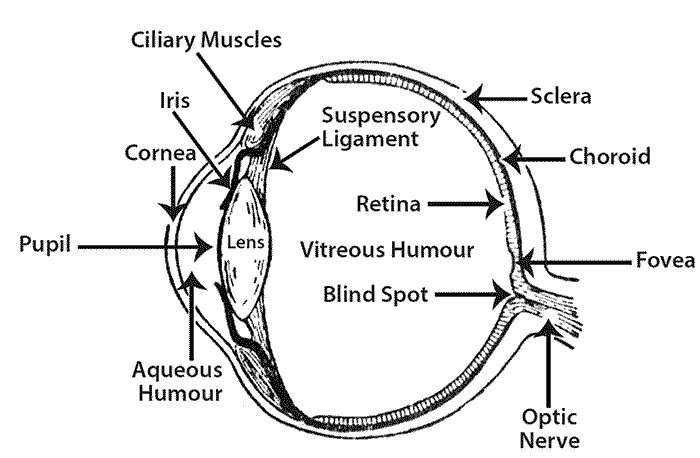
\includegraphics[height=6cm]{human_eye}
\caption{ساختار چشم انسان}
\label{fig:human_eye}
}
\end{figure}

\section{شبکیه}
ادراک بینایی از شبکیه‌ی چشم آغاز می‌شود. پرتوهای منعکس شده از یک جسم با عبور از عدسی به شبکیه می‌رسند و طرحی را در پشت چشم ترسیم می‌کنند که توسط گیرنده‌های حسی به سیگنال‌های الکتریکی تبدیل خواهند شد که ارسال آنها به مراکز بالاتر در مغز خط سیر بینایی را آغاز می‌کند. 

مطالعه‌ی شبکیه به دو دلیل اصلی از اهمیت بسیاری برخورد دارد است. نخست اینکه نقش بلامنازعی در کمک به درک انتقال اطلاعات حسی و همچنین به عنوان یکی از مراحل اصلی بینایی دارد. از همین رو گیرنده‌های نوری در شبکیه‌ی چشم از نظر حجم مطالعه‌ی صورت گرفته روی آنها شاید یکی از شناخته شده‌ترین سلول‌های حسی محسوب می‌شوند. دوم اینکه برخلاف سایر عناصر حسی مانند گیرنده‌های لامسه یا ساختار حلزونی در گوش، شبکیه عضوی جانبی نبوده و بلکه بخشی از دستگاه عصبی مرکزی محسوب می‌گردد. شباهت ساختاری سیناپس‌های شیمیایی شبکیه به عناصر دیگر تشکیل دهنده‌ی دستگاه عصبی مرکزی و سادگی نسبی ساز و کار آن نیز از عوامل انگیزش مطالعه‌ی آنها محسوب می‌شود. 

نور بازتاب شده از محیط پیرامون از طریق عدسی\footnote{\lr{Lens}} و قرنیه\footnote{\lr{Cornea}} متمرکز شده و بعد از عبور از مایع زجاجیه\footnote{\lr{Vitreous body}} که فضای حفره چشم را پر کرده و شکل کروی چشم را حفظ می‌کند به گیرنده‌های نوری در شبکیه می‌رسد. شبکیه در جلوی یک لایه از سلول‌های اپیتلیوم رنگدانه‌دار\footnote{\lr{Pigment epithelial cells}} که پشت چشم را پوشانده‌اند قرار دارد. سلول‌های بافت اپیتلیوم که رنگدانه‌ی سیاه بسیاری دارند، هر نوری که به شبکیه برخورد نکرده را جذب می‌کنند. این لایه از انعکاس نور به پشت چشم و بازتاب آن که می‌تواند باعث کاهش وضوح تصویر شود جلوگیری می‌کند. شبکیه داخلی‌ترین لایه‌ی چشم بوده و از سلول‌های گیرنده‌ی نوری (مخروطی\footnote{\lr{Cone cell}} و استوانه‌ای\footnote{\lr{Rod cell}}) تشکیل شده است. شبکیه بسیار نازک بوده (حدود نیم میلی‌متر) و حدود ۷۵٪ سطح کره‌ی چشم را می‌پوشاند. لکه‌ی زرد\footnote{\lr{Macula}} بخشی از شبکیه است که در امتداد محور نوری کره‌ی چشم در راستای مردمک و در نزدیکی مرکز شبکیه قرار داشته و بیشترین حساسیت به نور را دارد و در دقت و تیزبینی چشم نقش مهمی ایفا می‌کند. گودی مرکزی\footnote{\lr{Fovea}} که بیشترین تراکم سلول‌های مخروطی چشم را دارد در لکه‌ی زرد قرار گرفته است. خروج عصب بینایی قسمتی از شبکیه را تشکیل می‌دهد که فاقد گیرنده‌های نوروی هست و در نتیجه این بخش که تحت عنوان نقطه کور\footnote{\lr{Blind spot}} شناخته می‌شود فاقد بینایی است.

\subsection{گیرنده‌های نوری}
شبکیه در چشم انسان از دو نوع سلول تشکیل شده است: استوانه‌ای و مخروطی. سلول‌های مخروطی مخصوص دید در روز\footnote{\lr{Photopic}} بوده و در نور قوی بیشتر فعال می‌شوند. در مقابل سلول‌های استوانه‌ای مخصوص دید در شب\footnote{\lr{Scotopic}} بوده و بیشتر در نور ضعیف تحریک شده و توانایی دیدن در تاریکی را فراهم می‌کنند. سلول‌های استوانه‌ای به رنگ‌ها حساسیت نشان نمی‌دهند و به همین جهت بینایی در تاریکی به صورت طیفی از خاکستری درک می‌شود. افرادی که سلول‌های مخروطی چشم‌شان را از دست می‌دهند نابینا محسوب می‌گردند در حالی که آسیب به سلول‌های استوانه‌ای منجر به شب‌کوری\footnote{\lr{Nyctalopia}} می‌شود. همچنین بیشترین تمرکز سلول‌های مخروطی در لکه‌ی زرد است، در حالی که بیشترین تمرکز سلول‌های استوانه‌ای در بخش‌های پیرامونی شبکیه است. در انسان سه گونه سلول مخروطی وجود دارد که هر کدام از آنها رگندانه‌های متفاوتی داشته و به طول موج مختلف (ولی دارای همپوشانی) از طیف نور، متناظر با رنگ‌های قرمز، سبز و آبی، واکنش نشان می‌دهند. 

\begin{figure}
\centering
{\footnotesize
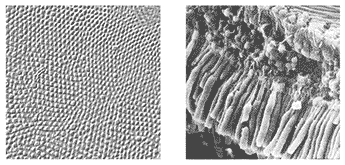
\includegraphics[height=6cm]{photoreceptors}
\caption[گیرنده‌های نوری]{چپ: برش مماس از گودی مرکزی که چینش گیرنده‌های مخروطی عادی شش‌ضلعی را نشان می‌دهد.\cite{kolb20webvision}
راست: نمای عمودی گیرنده‌های نوری\cite{corenward}
}
\label{fig:photoreceptors}
}
\end{figure}

\subsection{سلول‌های گانگلیون}
سلول‌های گانگلیون\footnote{\lr{Ganglion cells}} (یا عقده‌ای) خروجی شبکیه‌ی چشم محسوب می‌شوند. کل دنیای تصویری که ما درک می‌کنیم در الگوهای آتش سلول‌های گانگلیون کد می‌شود. سلول‌های گانگلیون ورودی خود را از نورون‌های بینابینی در شبکیه دریافت کرده و آکسون آنها از طریق عصب باصره\footnote{\lr{Optic nerve}} به بخش‌های بالاتر در مغز، به خصوص هسته‌ی زانویی جانبی\footnote{\lr{Lateral geniculate nucleus}} منتقل می‌شود. بین گیرنده‌های نوری و سلول‌های گانگلیون سه گروه نورون بینابینی\footnote{\lr{Interneurons}} وجود دارند: سلول‌های دوقطبی\footnote{\lr{Bipolar cells}}، سلول‌های افقی\footnote{\lr{Horizontal cells}} و سلول‌های آماکرین\footnote{\lr{Amacrine cells}}. این سلول‌ها صرفا سیگنال الکتریکی حاصل از تحریک گیرنده‌های نوری را منتقل نمی‌کنند، بلکه به گونه‌ای سیگنال‌های چند گیرنده‌ی نوری را با هم ترکیب می‌کنند که پاسخ الکتریکی به طور دقیق به طرح‌های فضایی و زمانی تحریک کننده‌ی نور وابسته و متکی باشد. 

\begin{figure}
\centering
{\footnotesize
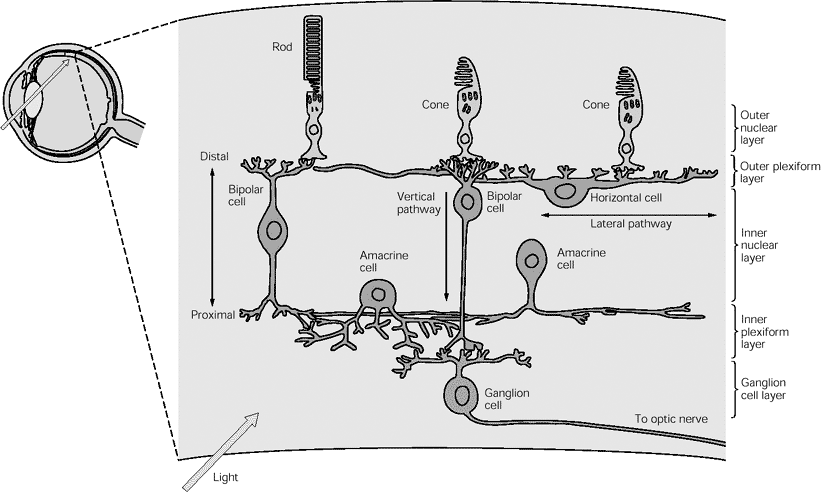
\includegraphics[width=16cm]{retina_neurons}
\caption[سه دسته کلاس نورونی در شبکیه]{\textbf{سه دسته کلاس نورونی در شبکیه:} گیرنده‌های نوری (استوانه‌ای و مخروطی) در لایه هسته خارجی قرار گرفته‌اند. نورون‌های بینابینی (دوقطبی، افقی و آماکرین) در لایه‌ی میانی و سلول‌های گانگلیون در لایه‌ی گانگلیون قرار دارند. گیرنده‌های نوری، سلول‌های دوقطبی و افقی با هم در لایه‌ی شبکه‌وارخارجی ارتباط سیناپسی برقرار می‌کنند. سلول‌های دوقطبی، آماکرین و گانگلیون نیز در لایه‌ی شبکه‌وار داخلی با هم ارتباط دارند. اطلاعات به صورت عمودی از گیرنده‌های نوری به سلول‌های دوقطبی و بعد به گانگلیون رفته و همچنین به صورت جانبی از طریق سلول‌های افقی در لایه‌ی شبکه‌وار خارجی و سلول‌های آماکرین در لایه‌ی شبکه‌وار داخلی جریان پیدا می‌کنند.\cite{kandel2000principles}}
\label{fig:retina_neurons}
}
\end{figure}

یافته‌های ارزشمند هارتلاین و گرانیت\cite{hartline1938response} که در سال ۱۹۶۷ جایزه‌ی نوبل را برای آنها به ارمغان آورد، بر اساس ثبت الکتریکی پاسخ تک نورون‌های گانگلیون نشان داد که پاسخ نورون‌های گانگلیون به یک ناحیه خاص از شبکیه که میدان تاثیر\footnote{\lr{Receptive field}} (\lr{RF}) نام دارد وابسته است. سازمان \lr{RF} یک سلول گانگلیون سه ویژگی دارد: \textit{مدور بودن\footnote{\lr{Circularity}}:} میدان تاثیر این سلول‌ها تقریبا مدور هستند. \textit{ساختار متضاد مرکز-اطراف\footnote{\lr{Antagonistic center-surround organization}}:} میدان تاثیر به دو بخش مدور مرکزی و حلقه‌ی محیطی تقسیم می‌شود. این زیرمیدان‌ها\footnote{\lr{Subfields}} با هم در تضاد بوده و تخاصم دارند؛ به این معنی که نور در حلقه‌ی محیطی در پاسخ سلول، اثر متمم نسبت به تاباندن نور در بخش مرکزی دارد. \textit{خط‌سیر‌های موازی داخل و خارج\footnote{\lr{Parallel on- and off-pathways}}:} دو نوع مختلف سلول گانگلیون داریم، سلول‌های «مرکز روشن - محیط خاموش» که به نقطه روشن با حلقه‌ی تاریک در دور بهترین پاسخ را داده و سلول‌های«مرکز خاموش - محیط روشن» که به عکس این محرک (نقطه‌ی تاریک با حلقه‌ی روشن) بهترین پاسخ را می‌دهد. این دو خط‌سیر موازی هستند؛ به این معنی که تقریبا به تعداد مساوی سلول مرکز روشن - محیط خاموش و مرکز خاموش - محیط روشن داشته و هر گیرنده‌ی نوری خروجی را به هر دو خط‌سیر می‌فرستد. در هر دو نوع سلول، پاسخی که با تابش به مرکز ایجاد می‌شود پاسخی را که در اثر تابش نور به محیط ایجاد می‌گردد را به طور کامل از بین می‌برد.

\begin{figure}
\centering
{\footnotesize
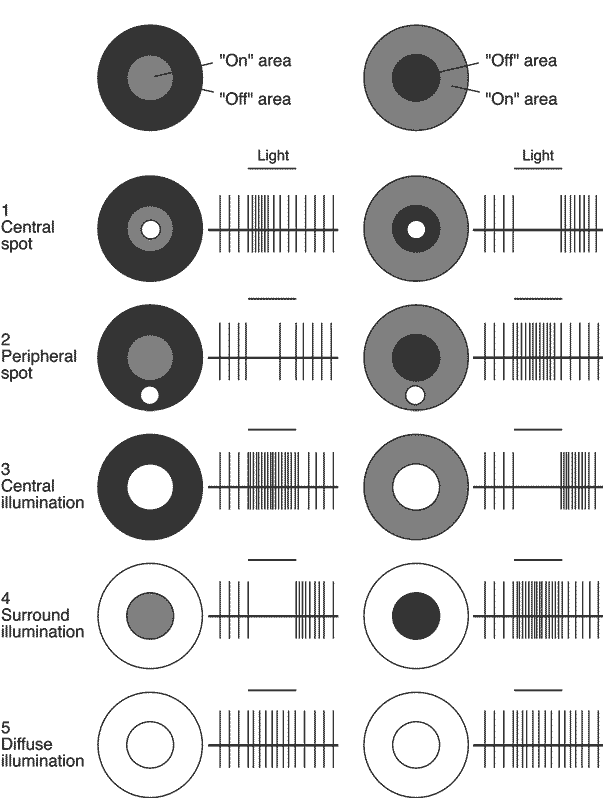
\includegraphics[width=10cm]{ganglion}
\caption[پاسخ سلول‌های گانگلیون]{سلول‌های گانگلیون در حالت بهینه به کنتراست در میدان تاثیرشان پاسخ می‌دهند.\cite{kandel2000principles}}
\label{fig:ganglion}
}
\end{figure}

اندازه‌ی میدان تاثیر سلول‌های گانگلیون یکنواخت نیست، بلکه بسته به فاصله از گودی مرکزی تغییر می‌یابد. در گودی مرکزی، مراکز میدان تاثیر قطری حدود چند دقیقه قوس دارند در حالی که در نواحی جانبی قرار گرفته در حواشی، میدان تاثیر حتی به بزرگی ۵ درجه نیز می‌رسد. هر درجه برابر ۶۰ دقیقه بوده و معادل حدود ۰/۲۵ میلی‌متر است.




\subsection{هسته‌ی زانویی جانبی}
هسته‌ی زانویی جانبی (\lr{LGN\footnote{\lr{Lateral Geniculate Nucleus}}}) مقصد اصلی سلول‌های گانگلیون است. \lr{LGN} یک زیرساختار از تالاموس\footnote{\lr{Thalamus}} (نَهَنج) می‌باشد. هر نیمکره از مغز دارای یک LGN می‌باشد. \lr{LGN} یک ساختار پیچیده‌ی ۶ لایه‌ای بوده و تعداد نورون آن تقریبا برابر تعداد کل سلول‌های گانگلیون است (حدود ۱/۵ تا ۱/۸ میلیون سلول). تالاموس وظیفه‌ی هماهنگی بین گیرنده‌های حسی و قشر مغز را داشته و با تقویت سیگنال‌های ورودی، آنها را به نواحی مختلف مغز رله می‌کند. 

\subsection{ستون‌های جهت‌گیری و میدان تاثیر \lr{V1}}
در شبکیه و همچنین \lr{LGN} میدان تاثیر سلول‌ها مدور بود. در قشر بینایی اولیه\footnote{\lr{Primary visual cortex}} یک تفاوت عمده در میدان‌های تاثیر صورت می‌گیرد: اکثر سلول‌ها میدان‌های تاثیری کشیده داشته و بهترین پاسخ را به خطوط، میله\footnote{\lr{Bar}} یا یکسری میله\footnote{\lr{Gratings}} که در یک جهت مرجح قرار گرفته‌اند می‌دهند. این یافته‌ها در نتیجه‌ی تحقیق پیشگامی است که برای دیوید هابل و تورستن ویزل جایزه‌ی نوبل را در سال ۱۹۸۱ به ارمغان آورد\cite{TJP19621601106}. 

بر اساس یافته‌های هابل و ویزل، سلول‌ها به دو دسته‌ی اصلی \textit{ساده} و \textit{پیچیده} تقسیم می‌شوند. سلول‌های ساده دو یا سه زیرمیدان کشیده‌ی جدا با پاسخ‌های روشن و خاموش متناوب داشته و یک محور جهت\footnote{\lr{Axis of orientation}} مشخص دارند. موثرترین محرک برای آنها، الگویی از تکه‌های روشن و خاموش است که با زیرمیدان‌های میدان تاثیر تلاقی کند؛ برای مثال یک خط یا میله در یک جهت مشخص. همان محرک با جهتی متعامد یا حتی مورب بدون پاسخ بوده یا صرفا منجر به پاسخی کوچک می‌شود. چنین محرکی برای یک سلول ساده‌ی دیگر با میدان تاثیر در همان موقعیت، بیشترین پاسخ را زمانی می‌دهد که جهت ارجح خودش را داشته باشد. بنابراین هر نقطه از میدان بینایی به صورت موازی توسط سلول‌های ساده که هر کدام جهت مرجح خود را دارند تحلیل می‌شود. جهت‌های ارجح در فواصل گسسته‌ی حدود $10^{\circ}$ قرار داشته و بنابراین حدود ۱۸ جهت مختلف در گستره‌ی $180^{\circ}$ داریم.

\begin{figure}
\centering
{\footnotesize
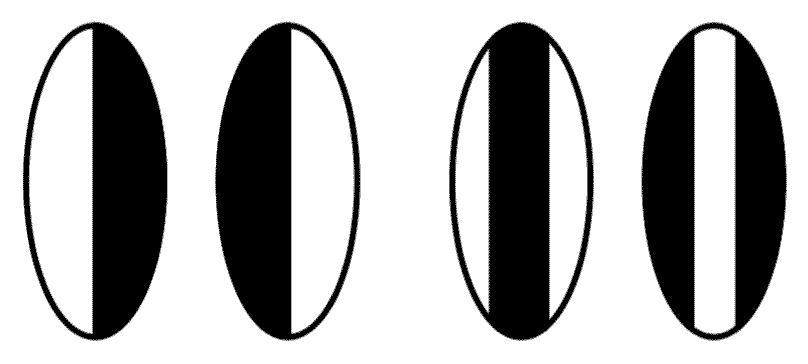
\includegraphics[width=6cm]{simple_cells}
\caption[میدان تاثیر سلول‌های ساده]{ترسیمی از میدان تاثیر سلول‌های ساده. نواحی روشن نمایانگر زیرمیدان‌های تحریکی و نواحی تاریک زیرمیدان‌های مهاری را نشان می‌دهند. میدان تاثیر سلول‌های درون‌جانداری به این منظمی نبوده ولی همین ساختار ابتدایی را دارد. سلول‌های ساده قادر به تشخیص خط در یک جهت، اندازه و محل مشخص هستند.}
\label{fig:simple_cells}
}
\end{figure}

\textit{سلول‌های پیچیده} یک جهت ارجح و همچنین میدان تاثیر بزرگتر دارند که، برخلاف سلول‌های ساده، نمی‌توان آن را به زیرمیدان‌های روشن و خاموش متمایز تقسیم کرد. این سلول‌ها همانند سلول‌های ساده به یک جهت خاص پاسخ می‌دهند ولی برخلاف آنها حساسیت کمتری نسبت به اندازه و محل قرارگرفتن محرک دارند. به عبارت دیگر، سلول‌های پیچیده حساس به زاویه و غیرحساس به اندازه و محل محرک می‌باشند. خصوصیات سلول‌های پیچیده از عمل ادغام\footnote{\lr{Pooling}} کردن سلول‌های ساده با موقعیت میدان تاثیر متفاوت، ولی با جهت یکسان بدست می‌آید. 

سلول‌های ساده و پیچیده در ستون‌های جهت‌گیری عمودی سازمان یافته‌اند. سلول‌های ساده و پیچیده در هر ستون، محور جهت یکسان داشته و میدان تاثیر آنها تقریبا در موقعیت مشابه است. هر ستون جهت‌گیری از سطح خارجی قشر شروع شده و تا ماده‌ی سفید ادامه می‌یابد و همه‌ی لایه‌های قشری را دربرمی‌گیرد. بنابراین یک جهت خاص در یک نقطه‌ی مشخص از میدان بینایی توسط سلول‌های ساده و پیچیده از سطوح مختلف انتزاعی در لایه‌های مختلف یک ستون جهت‌گیری صورت می‌گیرد.

\begin{figure}
\centering
{\footnotesize
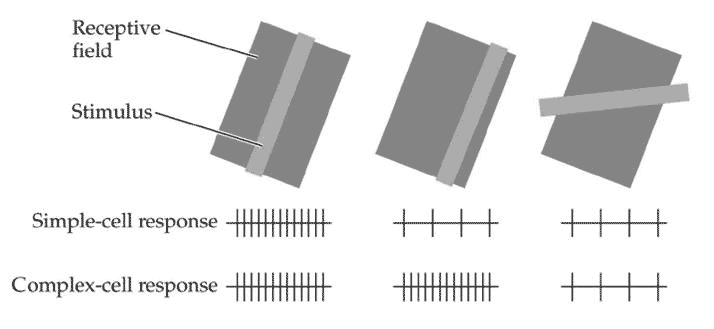
\includegraphics[width=10cm]{complex_cells}
\caption{تفاوت پاسخ سلول‌های ساده و پیچیده}
\label{fig:complex_cells}
}
\end{figure}

خط‌سیر بینایی پس از قشر بینایی اولیه به دو مسیر پشتی\footnote{\lr{Dorsal stream}} و شکمی\footnote{\lr{Ventral stream}} تقسیم می‌شود. در طول هر کدام از این خطوط‌سیر، مغز به اطلاعات خاصی از تصویر دست پیدا می‌کند. مسیر پشتی برای یافتن کجایی\footnote{\lr{Where pathway}} شی و مسیر شکمی برای یافتن چیستی\footnote{\lr{What pathway}} شی است. 

\section{خط‌سیر بینایی}
میدان دید، همانطور که در شکل \ref{fig:visual_pathway} مشاهده می‌کنید، از دو قسمت تشکیل شده است: \textit{منطقه دید دوچشمی} که توسط هر دو چشم دریافت می‌شود و \textit{منطقه دید یک چشمی} که صرفا توسط یکی از چشم‌ها دریافت می‌شود. 

وقتی یک شی در منطقه‌ی یک چشمیِ راست قرار بگیرد، بازتاب نور از آن به نیمه سمت بینی شبکیه چشم راست می‌رسد. اگر شی در منطقه‌ی دوچشمیِ میدان دید قرار داشته باشد، بازتاب نور به نیمه‌ی سمت بینی شبکیه‌ی چشم راست و همچنین منطقه‌ی نیمه گیجگاهی چشم چپ خواهد رسید\cite{kolb20webvision}. ورودی‌هایی که به نیمه سمت بینی شبکیه می‌رسند پس از تطبیق به تالاموس (مرکز پردازش داده‌های حسی) سمت مقابل رفته و سپس به قشر مغز نیم‌کره‌ی مقابل می‌روند؛ اما ورودی رسیده به منطقه نیمه گیجگاهی بدون تطبیق به تالاموس و سپس قشر نیم‌کره‌ی سمت خود می‌روند. 

\begin{figure}
\centering
{\footnotesize
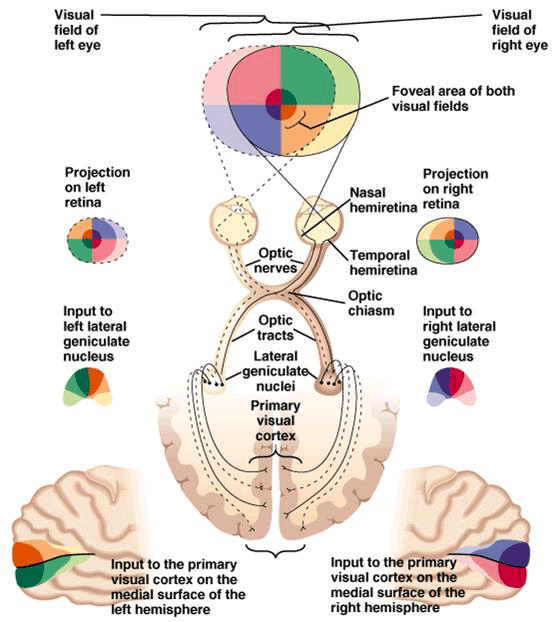
\includegraphics[width=10cm]{visual_pathway}
\caption{محل پردازش بخش‌های مختلف میدان دید در قشر بینایی مغز}
\label{fig:visual_pathway}
}
\end{figure}

اگر جسمی در سمت راست میدان بینایی قرار بگیرد، به روی نیمه گیج‌گاهی چشم چپ و همچنین بر روی نیمه سمت بینی چشم راست ظاهر می‌شود. فیبر‌های نیمه سمت بینی شبکیه در چلیپای نوری\footnote{\lr{Optic chiasm}} به سمت مقابل رفته و فیبر‌های نیمه گیج‌گاهی شبکیه‌ی هر طرف به تالاموس خود می‌روند. بنابراین در این حالت محرک در سمت راست خط مرکزی عمودی قرار گرفته است و اطلاعات آن از طریق نیمه گیج‌گاهی چشم چپ به تالاموس چپ و از طریق نیمه سمت بینی شبکیه‌ی چشم راست (بعد از تقاطع فیبر‌ها در چلیپا‌ی نوری) به قشر سمت چپ انتقال می‌یابد. به این ترتیب همه اطلاعات جسمی که در سمت راست میدان دید قرار گیرد در نیمکره‌ی چپ مغز و همه اطلاعات جسمی که در سمت چپ باشد در نیمکره‌ی سمت راست مغز پردازش می‌شود.  همانطور که تبیین شد، سازمان‌بندی بینایی بر اساس چشم چپ و راست صورت نگرفته بلکه بر اساس میدان بینایی و دو نیمه‌ی چپ و راست آن می‌باشد که اطلاعات به نیم‌کره‌ی راست یا چپ می‌رود. 

\section{ساختار قشر بینایی مغز}
قشر مغز\footnote{\lr{Cerebral cortex}} لایه‌ی نازک خاکستری پوشاننده‌ی سطح مغز است که از سلول‌های عصبی تشکیل شده است و ضخامتی بین ۲ تا ۴ میلی‌متر دارد. این قشر وظایف پیچیده‌تر مغز همانند حافظه، یادگیری، حل مسئله، طرح ریزی، پردازش زبان، بینایی، شنوایی و حرکت را تحت کنترل دارد. قشر مغز از لحاظ آناتومی به دو نیم‌کره و چهار لوب (شکل \ref{fig:cerebral_cortex}) تقسیم می‌شود:

\begin{itemize}
\item
\textbf{لوب گیج‌گاهی\footnote{\lr{Temporal lobe}}:}
ذخیره حافظه جدید، پردازش اطلاعات حواس شنوایی، درک زبان و سازماندهی از کارکردهای این لوب از مغز هستند.

\item
\textbf{لوب آهیانه‌ای\footnote{\lr{Parietal lobe}}:}
حس لامسه، ادراک فضایی، ادراک دیداری، بازشناسی اندازه‌ها، رنگ و اشکال از یکدیگر و احساس درد از کارکردهای این لوب است. این قسمت همچنین در نوشتن و بخشی از جنبه‌های خواندن نیز دخیل می باشد. 

\item
\textbf{لوب پیشانی\footnote{\lr{Frontal lobe}}:}
محتوای شخصیتی، چاره‌یابی، هیجانات، تمرکز، داوری، سخن گفتن و حرکات ارادی از کارکردهای لوب پیشانی محسوب می‌شوند. این بخش در ارتباط با توابع شناختی سطح بالا مانند استدلال و قضاوت است.

\textbf{لوب پس‌سری\footnote{\lr{Occipital lobe}}:}
این لوب عقب‌ترین بخش مغز است و قسمت کوچکی از سطح پشتی-جانبی آن را تشکیل می‌دهد. لوب پس‌سری دربرگیرنده‌ی قشر اولیه بینایی بوده و مرکز پردازش اطلاعات دیداری در پستانداران محسوب می‌شود. 
\end{itemize}


\begin{figure}
\centering
{\footnotesize
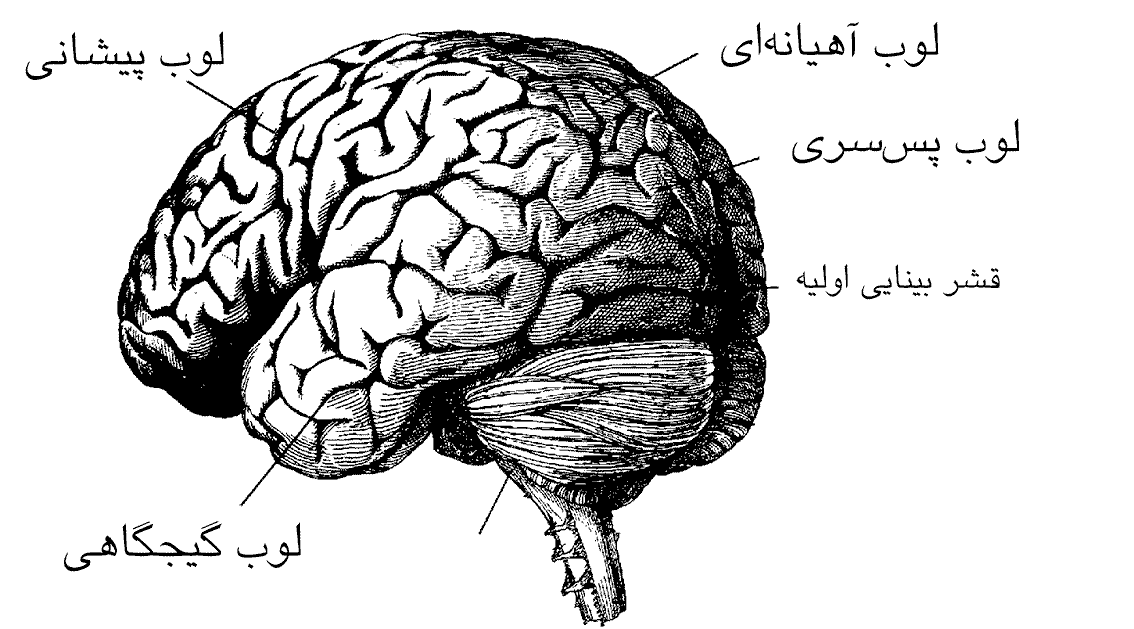
\includegraphics[width=12cm]{cerebral_cortex}
\caption{قشر مغز و لوب‌های مختلف آن}
\label{fig:cerebral_cortex}
}
\end{figure}

شکل \ref{fig:dorsal_ventral_pathways} تقسیم‌بندی بخش‌های مختلف قشر بینایی مغز را نشان می‌دهد که \lr{V1} و \lr{V2} بزرگترین بخش‌ها هستند. فیزیولوژیست‌ها با مطالعه‌ی این قشر گذرگاه‌های متفاوتی را کشف کرده‌اند. اطلاعاتی که از تالاموس به \lr{V1} می‌رسد، در دو مسیر جداگانه و به صورت مستقل پردازش می‌شود:

\begin{itemize}
\item
\textbf{گذرگاه چیستی\footnote{\lr{What stream}}:}
گذرگاه چیستی اطلاعات مربوط به چیستی اشیا مانند رنگ، شکل و بافت را پردازش می‌کند. لوب پس‌سری و گیج‌گاهی در این گذرگاه دخیل بوده و در مسیر \lr{V1}، \lr{V2}، \lr{V4}، \lr{AIT} و \lr{PIT} قرار دارند. 

\textbf{گذرگاه کجایی\footnote{\lr{Where stream}}:}
گذرگاه کجایی اطلاعات مربوط به مشخصات فضایی شی مانند حرکت  و عمق شی را پردازش می‌کند. لوب پس‌سری و آهیانه‌ای در این گذرگاه دخیل بوده و در مسیر \lr{V1}، \lr{V2}، \lr{V3}، \lr{MT} و \lr{MST} قرار دارند. 
\end{itemize}

به طور مثال، اگر یک فرد یک اتومبیل در حال حرکت را مشاهده کند، با کمک مسیر چیستی، اتومبیل بودن آن و به وسیله‌ی مسیر کجایی، حرکت و جهت آن تشخیص داده می‌شود. 
گذرگاه چیستی و گذرگاه کجایی دو مصداق پردازش موازی، به معنای توزیع همزمان اطلاعات در گذرگاه‌های عصبی مغز، هستند. علی رقم موازی بودن گذرگاه چیستی و کجایی، اتصال آنها منجر به ادغام اطلاعات حسی و ترسیم تصویر کاملی از دنیای بیرون می‌شود. 

\begin{figure}
\centering
{\footnotesize
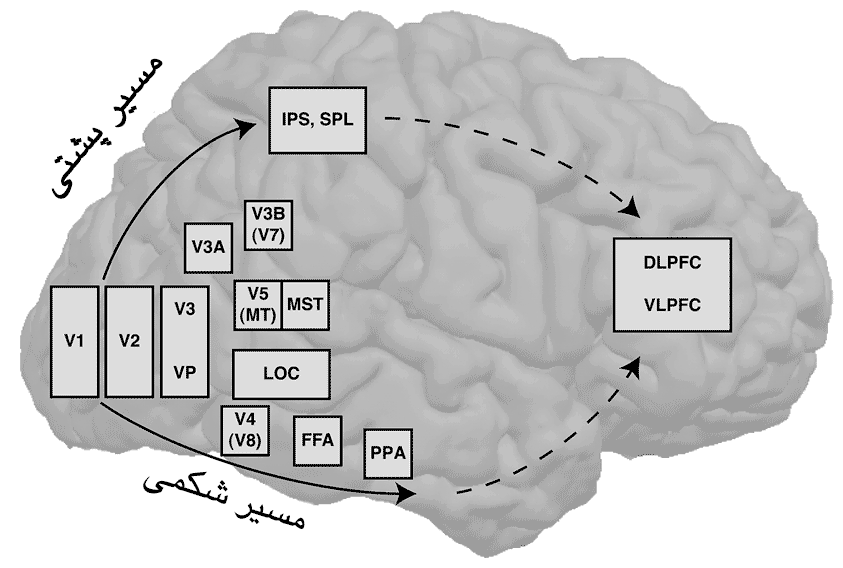
\includegraphics[width=12cm]{dorsal_ventral_pathways}
\caption[بخش‌های اصلی قشر بینایی]{بخش‌های اصلی قشر بینایی: نواحی بینایی در مغز در مسیر‌های پشتی (پس‌سری و گیج‌گاهی) و شکمی (پس‌سری و آهیانه‌ای) سازمان یافته‌اند. فرضیات نشان می‌دهند که هر دوی این مسیرها به قشر پیش‌پیشانی ختم می‌شوند. لازم به ذکر است که این مسیرها تنها از اتصالات پیش‌خور (رو‌به‌جلو) تشکیل نشده و حجم زیادی از اتصالات بازخورد وجود دارد.}
\label{fig:dorsal_ventral_pathways}
}
\end{figure}
\subsection{ناحیه \lr{V1}}
پیشتر اشاره شد که شبکیه تصویر را به نقاطی که میزان درخشندگی مشخصه‌ی خاصه‌ی آنها می‌باشد تجزیه می‌کند. نورون‌های قشر بینایی در مقابل می‌بایست اطلاعات تجزیه شده را بازسازی کنند. اولین قدم در بازسازی در قشر \lr{V1} (ناحیه‌ی ۱۷ در تقسیم‌بندی برادمن\footnote{\lr{Brodmann areas}}؛ شکل \ref{fig:brodmann}) صورت می‌گیرد. این ناحیه بزرگترین قسمت از قشر بینایی مغز (حدود ۲۰٪) را تشکیل می‌دهد. سلول‌های موجود در این ناحیه به لبه‌ها و خطوط پاسخ می‌دهند. به عبارت دیگر هر سلول به امتداد جهت خاصی از محرک در موقعیت مشخصی از میدان بینایی پاسخ می‌دهد. به این سلول‌ها، سلول‌های گزینش‌پذیر نسبت به جهت\footnote{\lr{Orientation selective}} گفته می‌شود. برای بازسازی تصویر، شناسایی جهت امتداد خطوط اولین قدم است. از این رو می‌توان ادعا کرد که دستگاه بینایی ما یک دستگاه تشخیص لبه بوده و به عبارتی شناسایی شی بر اساس لبه‌های تشکیل دهنده‌ی تصویر آن صورت می‌پذیرد. در ناحیه‌ی \lr{V1} نورون‌ها دارای میدان تاثیر به نسبت کوچکی هستند. اندازه‌ی میدان تاثیر برای سلول‌های \lr{V1} در نقطه‌ی مرکزی دید حدود یک درجه ($7\times 7$ پیکسل) می‌باشد. 

\begin{figure}
\centering
{\footnotesize
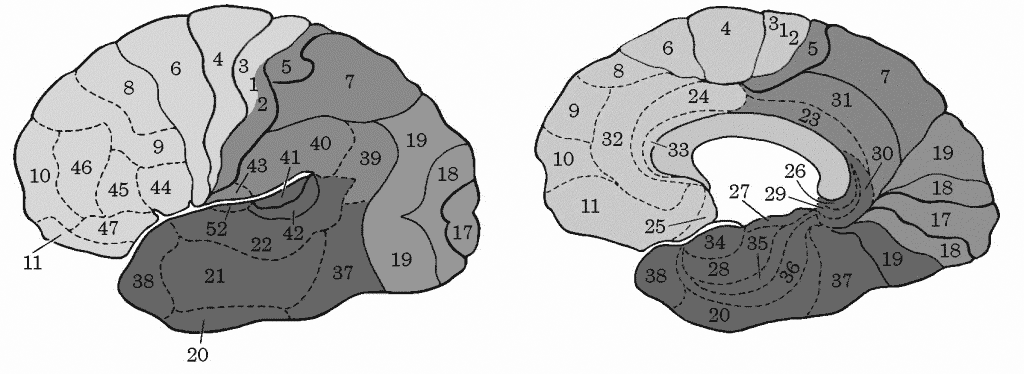
\includegraphics[height=5cm]{brodmann}
\caption[تقسیم‌بندی Brodmann]{تقسیم‌بندی برادمن: سمت چپ نمای جانبی و سمت راست نمای شکاف میانی را نشان می‌دهد. \lr{V1} ناحیه‌ی ۱۷ این تقسیم‌بندی است.}
\label{fig:brodmann}
}
\end{figure}

همانطور که پیشتر بیان شد، دو نوع سلول تشکیل دهنده‌ی \lr{V1}، نورون‌های ساده و پیچیده، وظیفه‌ی شناسایی جهت محرک را انجام می‌دهند. شکل \ref{fig:V1_stimuli} نمونه‌ای از میدان تاثیر یک سلول ساده را بررسی می‌کند. نقاط مثبت (منفی) نمایانگر نقاط تحریکی (مهاری) هستند. به عبارت دیگر نقاط منفی فعالیت نورون را مهار کرده و نقاط مثبت فعالیت نورونی را تشدید می‌کند. مرز مشخصی که بین این نقاط در میدان تاثیر مشاهده می‌شود جهت مورد گزینش نورون را نشان می‌دهد. طبیعتا نورونی مانند نورون شکل \ref{fig:V1_stimuli} که به میله‌ی عمودی بهترین پاسخ را می‌دهد به میله‌های مورب پاسخی نداده یا پاسخ ضعیفی خواهد داد. 

\begin{figure}
\centering
{\footnotesize
\includegraphics[height=7cm]{V1_stimuli}
\caption[میدان تاثیر یک سلول ساده در \lr{V1}]{میدان تاثیر یک سلول ساده در \lr{V1}: بیشترین پاسخ سلول را در حالتی که یک میله روشن در جهت ارجح (عمودی) قرار گرفته باشد داریم. نقاط روشن پاسخی نداشته یا باعث پاسخ‌های ضعیف می‌شوند. نقطه روشن اگر در مرکز برانگیزنده باشد صرفا پاسخ ضعیف برانگیزنده و اگر در حاشیه‌ی مهارکننده باشد باعث پاسخ مهاری ضعیف می‌شود. اگر نور روی کل میدان تاثیر پخش شده و آن را بپوشاند پاسخی نخواهیم داشت.\cite{kandel2000principles}}
\label{fig:V1_stimuli}
}
\end{figure}

آرایه‌ای از سلول‌ها در قشر بینایی، محرک‌های یک نقطه از شبکیه را در میدان تاثیر خود در جهت‌های مختلف دریافت کرده (شکل \ref{fig:simple_rf2}) و بنابراین هر کدام در جهت‌های متفاوتی حساس هستند. همچنین سلول‌های ساده نواحی تحریکی و مهاری در میدان تاثیر خود دارند که البته بزرگتر از میدان تاثیر سلول‌های گانگلیون می‌باشد. می‌توان عملکرد این سلول‌ها را به این نحو تبیین کرد که فیلترهای لبه‌یابی هستند که با اعمال روی تصویر، لبه‌ها در جهات مختلف را شناسایی می‌کنند. تمایز سلول‌های ساده با سلول‌های پیچیده در میزان حساسیت آنها به موقعیت مکانی لبه است. نورون‌های ساده به موقعیت مکانی محرک بسیار حساس بوده و با تغییر موقعیت لبه پاسخ آنها به شدت افت می‌کند. این در حالی است که سلول‌های پیچیده، در یک محدوده‌ی مکانی مشخص و بزرگتر از میدان تاثیر سلول‌های ساده، فارغ از موقعیت به لبه با جهت ارجحشان پاسخ می‌دهند. این خصوصیات هابل و ویزل را به تبیین نظریه‌ی پردازش سلسله مراتبی این سلول‌ها واداشت\cite{TJP19621601106,hubel1968receptive}.

\begin{figure}
\centering
{\footnotesize
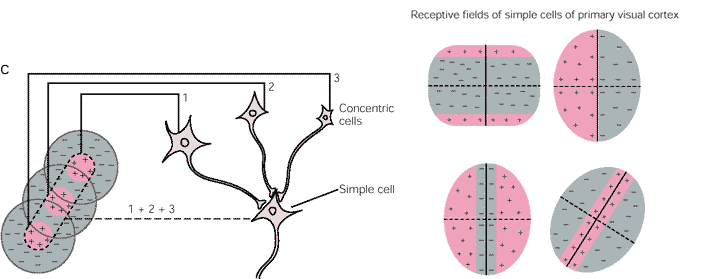
\includegraphics[height=5cm]{simple_rf2}
\caption[اتصال سلول‌های \lr{LGN} به سلول‌های ساده و تشکیل میدان تاثیر]{اتصال سلول‌های \lr{LGN} به سلول‌های ساده و تشکیل میدان تاثیر: طبق نظریه‌ی هابل و ویزل، یک نورون ساده در قشر مغز، اتصالات همگرای برانگیزنده از سه یا بیشتر نورون داخل‌مرکز دریافت می‌کند که با هم می‌توانند نور قرار گرفته در راستای یک خط در شبکیه را نمایش دهند. در نتیجه میدان تاثیر یک سلول ساده بیضوی و کشیده می‌نماید. حلقه‌ی مهاری حاشیه‌ای نیز توسط سلول‌های خارج‌از‌مرکز تامین می‌شود که میدان تاثیرشان در همسایگی سلول‌های داخل‌مرکز است.\cite{kandel2000principles}}
\label{fig:simple_rf2}
}
\end{figure}

نکته‌ی قابل توجه دیگر در مورد نورون‌های \lr{V1} ترتیب قرار گیری آنها در قشر اولیه بینایی بر حسب جهت‌گیری آنها است که نورون‌های با جهت‌گیری نزدیک به هم، در کنار یکدیگر قرار گرفته‌اند\cite{hubel1969anatomical}. اگر یک الکترود ثبت نورونی را به صورت عمودی در قشر مغز فرو کنیم، میدان تاثیر اندازه‌گیری شده از سطح خارجی قشر تا رسیدن به ماده‌ی سفید مشابه خواهد بود. بنابراین قشر بینایی اولیه تحت یک سری ستون باریک که میدان تاثیر مشابه دارند بسته‌بندی شده است\cite{goebel2004visual}. به این خوشه‌های هم میدان تاثیر «ستون‌های قشری» گفته می‌شود\cite{hubel1977ferrier}. ستون‌های قشری از جمله اصول ساختاری هستند که در جای جای مغز به آنها برمی‌خوریم. چنین سازمان‌های ستونی در بخش‌های مختلف قشر مغز، از قشر حسی لامسه‌ای گرفته تا قشر شنوایی یافت می‌شوند. این نورون‌ها طیف گسترده‌ای از زوایای بین صفر تا ۱۸۰ درجه را تشخیص می‌دهند. 

ستون‌های جهت‌گیری قرار گرفته در کنار هم، در جهت ارجحشان تفاوتی گسسته در حدود $10^\circ$ مشاهده می‌شود. هابل و ویزل مفهوم اَبَرستون\footnote{\lr{Hypercolumns}} را معرفی کردند که مجموعه‌ای از ستون‌ها هستند که به همه‌ی جهت‌های ممکن در یک ناحیه‌ی مشخص و در هر دو چشم پاسخ می‌دهند‌. بنابراین یک ابرستون می‌تواند تحلیل کاملی (کامل از منظر خصوصیات تحلیل شده در \lr{V1}) از یک ناحیه‌ی خاص ارائه دهد. 
حباب‌ها در لایه‌ی ۲ و ۳ قرار گرفته و جهت‌گیری نمی‌کنند. حباب‌ها\footnote{\lr{Blobs}} گروه‌های نورونی هستند که مستقیما از \lr{LGN} ورودی می‌گیرند و در پردازش رنگ نقش دارند. 



\begin{figure}
\centering
{\footnotesize
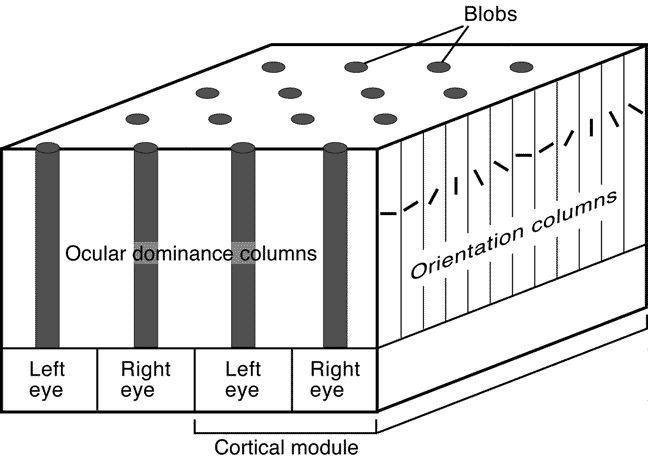
\includegraphics[height=6cm]{hypercolumns2}
\caption[چیدمان نورون‌های \lr{V1} با جهت‌گیری‌های متفاوت]{چیدمان نورون‌های \lr{V1} با جهت‌گیری‌های متفاوت\cite{goebel2004visual}}
\label{fig:hypercolumns2}
}
\end{figure}

\section{سطوح بالاتر بینایی}
نواحی بسیار دیگری از قشر بینایی به جز \lr{V1} وجود دارند که بیشتر یا انحصارا درگیر بینایی هستند و تنها تعدادی از آنها به خوبی مطالعه شده‌اند و دانش ما از آنها نسبتا کم است. ناحیه‌ی بینایی ثانویه (\lr{V2})‌ مشابه \lr{V1} همه گروههای عملیاتی از نورون‌ها را دارد. نواحی دیگر \lr{V3}-\lr{V5} عملکرد‌های خاص‌تری دارند. مهمترین اصل پردازش بینایی در نواحی بالاتر، پردازش موازی جنبه‌های مختلف بینایی در نواحی متفاوت و تفکیک‌شده است. همانگونه که اشاره شد، پیشنهاد شده است که بخش‌های غیر \lr{V1} (قشر فرامخطط\footnote{\lr{Extrastriate cortex}}) تحت دو گذرگاه شکمی و پشتی دسته‌بندی شوند. 

\subsection{ناحیه‌ی \lr{V2}}
دومین ناحیه از سلسله مراتب پردازش، ناحیه‌ی \lr{V2} (شامل نواحی ۱۸ و ۱۹ برادمن) است که قشر اولیه بینایی را احاطه کرده و مانند \lr{V1} یک ساختمان توپوگرافی دارد. \lr{V2} مانند \lr{V1} به نواحی خبره \lr{V3}-\lr{V5} خروجی می‌دهد. \lr{V1} بخش اعظمی از اتصالاتش را به \lr{V2} می‌فرستد و \lr{V2} ورودی نقطه به نقطه از \lr{V1} دارد. \lr{V2} همچنین اتصالات بازخوردی قوی به \lr{V1} می‌فرستد. مسیر‌های رنگ، شکل و حرکت که در \lr{V1} شکل می‌گیرد، در \lr{V2} امتداد می‌یابد. به جهت تفکیک این نورون‌ها می‌توان اشاره کرد که نورون‌های مسیر رنگ در \lr{V2} نسبت جهت حساس نیستند، در صورتی که نورون‌های مسیر شکل در \lr{V2} نسبت به جهت محرک حساسند. نیمی از این نورون‌ها به انتهای لبه‌ها و خطوط پاسخ می‌دهند. مسیر حرکت زمانی که تنها یک چشم تحریک می‌شود پاسخ ضعیفی نشان می‌دهد اما در صورتی که اطلاعات از هر دو چشم دریافت شود، پاسخ قوی‌تری مشاهده می‌شود. 

\begin{figure}
\centering
{\footnotesize
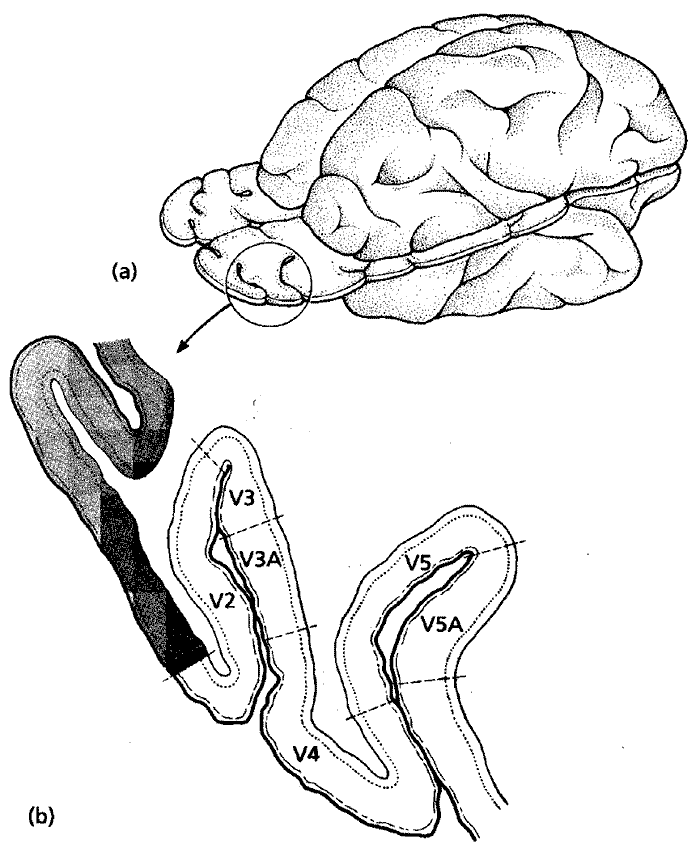
\includegraphics[height=9cm]{prestriate_cortex}
\caption[قشر اولیه‌ی بینایی (به رنگ طوسی) و نواحی فرامخطط شامل \lr{V2}-\lr{V5}]{قشر اولیه‌ی بینایی (به رنگ طوسی) و نواحی فرامخطط شامل \lr{V2}-\lr{V5}\cite{zeki1993vision}}
\label{fig:prestriate_cortex}
}
\end{figure}

\subsection{ناحیه‌ی \lr{V4}}
ناحیه‌ی \lr{V4} در موقعیت قدامی نسبت به \lr{V2} و خلفی نسبت به \lr{PIT} قرار گرفته است. \lr{V4} سومین ناحیه‌ی قشری در مسیر شکمی بوده و از \lr{V2} ورودی گرفته و اتصالات خروجی قوی به \lr{PIT} دارد. همچنین اتصالات ورودی مستقیم از \lr{V1} دارد و اتصالات خروجی ضعیف‌تری بین آن و \lr{V5} وجود دارد. این ناحیه اولین ناحیه در جریان شکمی است که مدولاسیون توجهی\footnote{\lr{Attentional modulation}} نشان می‌دهد. تحقیقات نشان داده که توجه گزینشی\footnote{\lr{Selective attention}} می‌تواند نرخ آتش در \lr{V4} را تا ۲۰٪ تغییر دهد. 

مشابه \lr{V2}، ناحیه‌ی \lr{V4} برای جهت، فرکانس فضایی و رنگ میزان‌سازی شده است اما برخلاف آن روی ویژگی‌های شی با پیچیدگی میانی، مانند اشکال هندسی، نیز حساس است. هنوز توصیف پارامتری از فضای میدان تاثیر این ناحیه ارائه نشده است اما می‌دانیم که \lr{V4} (برخلاف \lr{IT}) نسبت به اشیای پیچیده، همانند تصویر صورت، حساس نیست. 

\begin{figure}
\centering
{\footnotesize
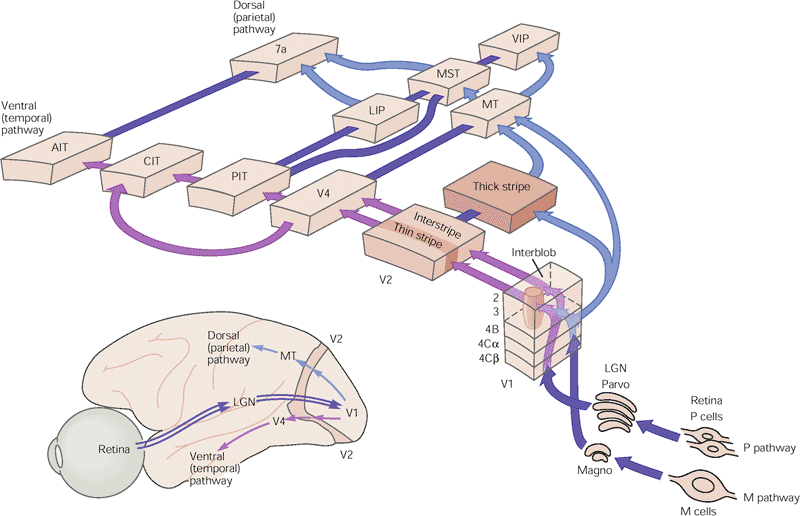
\includegraphics[height=9cm]{higher_areas}
\caption[نواحی بالاتر قشر بینایی و دو گذرگاه شکمی و پشتی]{نواحی بالاتر قشر بینایی و دو گذرگاه شکمی و پشتی\cite{kandel2000principles}}
\label{fig:higher_areas}
}
\end{figure}

\subsection{قشر \lr{IT}}
قشر گیجگاهی تحتانی (\lr{IT})، متشکل از قشرهای \lr{PIT}، \lr{CIT} و \lr{AIT}، بر اساس نتایج مشاهدات تجربی، به عنوان آخرین ناحیه‌ی درگیر در مسیر شکمی بینایی شناخته می‌شود. \lr{IT} محرک بینایی از اشیای داخل میدان دید را پردازش کرده و در حافظه و همچنین ادراک محرکی که توسط نواحی ، \lr{V2}، \lr{V3} و \lr{V4} در لوب پس‌سری تقویت شده‌اند نقش دارد. این ناحیه مسئول تولید «چیستی» از محرک‌های بینایی است و به عبارت دیگر بر اساس رنگ و فرم شی و مقایسه‌ی آن با اطلاعات ذخیره شده در حافظه، آن را شناسایی می‌کند.